%%%%%%%%%%%%%%%%%%%%%%%%%%%%%%%%%%%%%%%%%%%%%%%%%%%%%%%%%%%%%%%%%%%%%%%%%%%%%%
%
% Topico     : Estilo de Informes - DMCC  
% Autor      : Ruben Carvajal Schiaffino
% Santiago de Chile, 13/9/2016
%
%%%%%%%%%%%%%%%%%%%%%%%%%%%%%%%%%%%%%%%%%%%%%%%%%%%%%%%%%%%%%%%%%%%%%%%%%%%%%%
% 
%
\documentclass{report}
%
%
%
\usepackage[spanish]{babel}
\usepackage{epsfig}
%
\usepackage{pdfpages}
\usepackage{float}
\usepackage{array}
\usepackage[utf8]{inputenc}
\usepackage[toc,header,title]{appendix}
\usepackage{graphicx}
\graphicspath{{./images/}}
%
\renewcommand*\thesection{\arabic{section}}
\newcommand \tab{\hspace*{25 pt}}
\newcommand \minitab{\hspace*{15 pt}}
\usepackage[pagestyles]{titlesec}
\titleformat{\chapter}[display]{\normalfont\bfseries}{}{0pt}{\Huge}
\newpagestyle{mystyle}
{\sethead[\thepage][][\chaptertitle]{}{}{\thepage}}
\pagestyle{mystyle}
%
\begin{document}
\begin{titlepage}
\begin{center}
%\psfig{figure=L-USACH-16.png,height=3cm,,}
\end{center}
\begin{center}
{\bf Departamento de Matem\'atica y Ciencia de la Computaci\'on}
\end{center}
\vspace{3cm}
\begin{center}
%%%%%%%%%%%%%%%%%%%%%%%%%%%%%%%%%%%%%%%%%%%%%%%%%%%%%%%%%%%%%%%%
%
% MODIFICAR. Despues del tag \bf se coloca el titulo del trabajo
%
{\Large \bf Primer examen}
%
%%%%%%%%%%%%%%%%%%%%%%%%%%%%%%%%%%%%%%%%%%%%%%%%%%%%%%%%%%%%%%%%
%
\end{center}
\begin{center}
%
%%%%%%%%%%%%%%%%%%%%%%%%%%%%%%%%%%%%%%%%%%%%%%%%%%%%%%%%%%%%%%%%
%
% MODIFICAR. Despues del tag \bf se coloca el semestre y año
%
{\large \bf Segundo Semestre 2018}
%
%%%%%%%%%%%%%%%%%%%%%%%%%%%%%%%%%%%%%%%%%%%%%%%%%%%%%%%%%%%%%%%%
%
\end{center}
\vspace{5cm}
\begin{tabular}{c l c}
%
%%%%%%%%%%%%%%%%%%%%%%%%%%%%%%%%%%%%%%%%%%%%%%%%%%%%%%%%%%%%%%%%
%
% MODIFICAR. En el primer campo colocar el nombre de la asignatura y su codigo
%            En el segundo campo colocar el nombre del autor
%
Algoritmos Distribuidos 26106 & ~~~~~~~~~~~~~~~~~ & Rafael A. Castillo L\'opez \\
%
%%%%%%%%%%%%%%%%%%%%%%%%%%%%%%%%%%%%%%%%%%%%%%%%%%%%%%%%%%%%%%%
%
% MODIFICAR. En el primer campo colocar el nombre de la carrera
%            En el segundo campo color direccion electronica
%
Licenciatura en Ciencia de la Computaci\'on & ~~ & rafael@trfs.me
%
%%%%%%%%%%%%%%%%%%%%%%%%%%%%%%%%%%%%%%%%%%%%%%%%%%%%%%%%%%%%%%%
%
\end{tabular}
\end{titlepage}

\chapter{Problema 1}

\section{Descripci\'on del problema}

\textbf{Enunciado} Haz un estudio del comportamiento del algoritmo que determina
la distancia de estrellas a partir de una matriz de intensidad de luz. La
implementaci\'on vista en clase recorre la matriz por filas. Construya una
implementaci\'on que la recorra por columnas y haga una comparaci\'on entre
las secuenciales y las paralelas. Recuerde que en clase se vieron dos metricas
para medir el rendimiento.

\section{Algoritmo}

El algoritmo por filas es el mismo visto en clase, y solo se necesitan
realizar cambios triviales para obtener la versión por columnas.

\section{Analis\'is de complejidad}

Ambos algoritmos secuenciales tienen complejidad lineal con respecto al numero
de elementos de la matriz de entrada. Es decir que para una matr\'iz de tamaño
$N \times M$. El algoritmo ser\'a $\mathcal{O}(MN)$.

\section{Experimentos}

Todos los experimentos se corrieron en un servidor con las siguientes
especificaciones

\begin{table}[H]
  \begin{tabular}{ >{\bf}l l }
  Procesador & Dos Intel Xeon Gold 6126 CPU @ 2.60GHz \\
  Numero de nucleos & 12 por procesador, 24 en total (48 hilos con Hyper Threading) \\
  Memoria ram & 128 GiB \\
  Sistema operativo & Ubuntu 16.04 x86-64 \\
  Memoria secundaria & SSD Samsung MZ7KM240HMHQ0D3 de 240 GiB\\
  Nucleo & Linux help 4.4.0-138
\end{tabular}
\end{table}

Se corr\'io cada algoritmo con matrices cuadradas de $N \times N$  para 
$N = 500, 1000, 1500 \ldots 9500, 10000 $. Como escalamos ambas
dimensiones de la matr\'iz al mismo tiempo y en las graficas de
rendimiento usaremos solo $N$ como eje $x$, para efectos de este experimento
el algoritmo se comportar\'a con complejidad $\mathcal{O}(N^2)$.

Cada punto de prueba se ejecut\'o con ambos algoritmos secuenciales, y
con ambos algoritmos paralelos con 3, 6, 12, 24, 48 y 96 hebras (empezamos de
3 ya que nuestro procesador tiene un n\'umero de nucleos multiplo de 3). Se
realizaron ademas 40 repeticiones del experimento y se tomo el valor mediano
para presentar resultados. Las tablas con los resultados resumidos se encuentran
en el ap\'endice.

En la figura \ref{fig:starperf} se muestran los tiempos de ejecución de ambos
algoritmos. Observamos que aunque teóricamente ambos algoritmos tengan
comportamientos asimptoticos exactamente iguales, ¡el algoritmo por columnas toma
casi el doble de tiempo que el algoritmo por filas! Esto probablemente se debe a
que la baja localidad de datos en el caso por columnas lleva a muchos fallos de
cache. Tambien se vé que los algoritmos paralelos ofrecen una mejora dramatica
sobre los secuenciales, aunque su comportamiento no sea tan estable.

\begin{figure}[h]
  \caption{Izquierda: rendimiento de los algoritmos por fila. Derecha: rendimiento
           de los algoritmos por columna.}
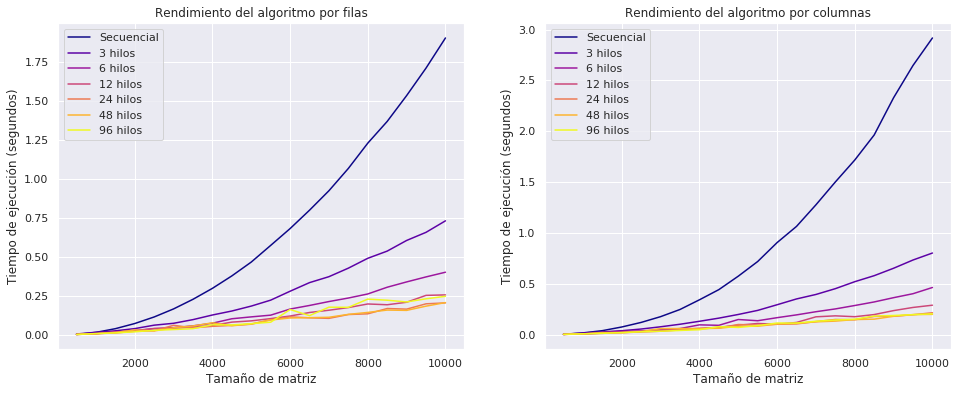
\includegraphics[width=\textwidth]{stars_perf}
\label{fig:starperf}
\end{figure}

La figura \ref{fig:starperfbar} nos muestra el rendimiento para el caso especifico
de una matríz de $10000 \times 10000$. Aqui se aprecia mejor como mejora el rendimiento con
mas hilos. Curiosamente podemos ver en el algoritmo por filas que el rendimiento
con 96 hilos es peor que el rendimiento con 48. 48 hilos es el maximo que el
procesador usado en las pruebas puede correr en paralelo (contando los nucleos
virtuales o HyperThreads). Esto no se presenta en la versión por columnas.
Hipotetizo que la razón de esto es que aunque el mas rápido algoritmo por filas
llegue a un cuello de botella ocasionado por el cambio de contexto entre hilos,
el algoritmo por columnas aún es limitado por su mas lento acceso a memoria.

\begin{figure}[H]
  \caption{Rendimiento para una matriz de $10000 \times 10000$}
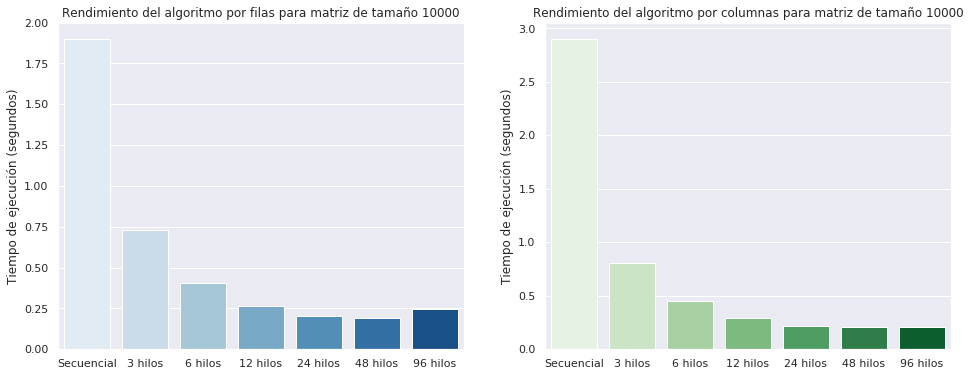
\includegraphics[width=\textwidth]{stars_1000_perf}
\label{fig:starperfbar}
\end{figure}

En el mapa de calor de la figura \ref{fig:staraccel} podemos ver la aceleración de
los algoritmos probados. Podemos ver la tendencia general de que la aceleración
crezca con el numero de hilos y el tamaño del problema, con la excepción previamente
mencionada del algoritmo por filas usando 96 hilos.

\begin{figure}[H]
  \caption{Mapa de calor de aceleración}
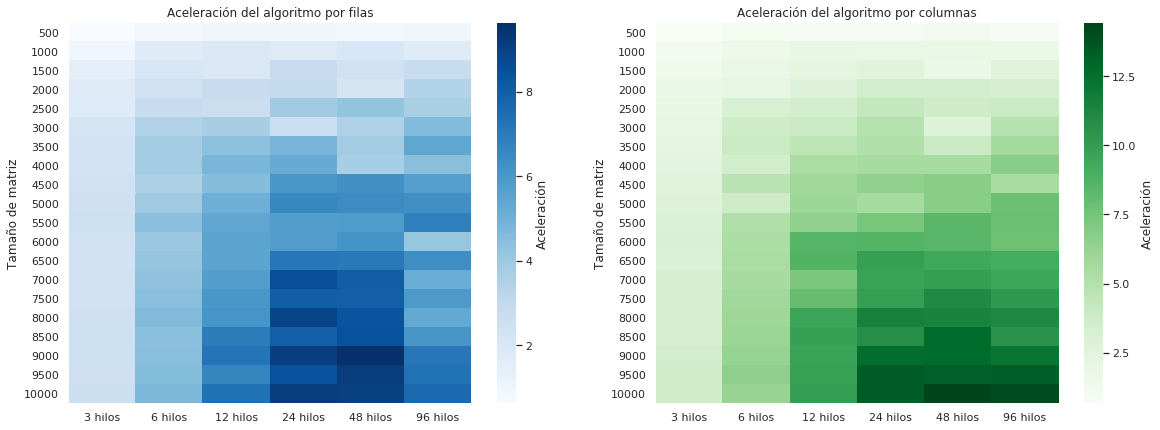
\includegraphics[width=\textwidth]{stars_accel}
\label{fig:staraccel}
\end{figure}

De nuevo acercandonos a nuestro caso extremo de la mátriz de $10000 \times 10000$ en
la figura \ref{fig:staraccelbar}, observamos que en ambos casos nuestra aceleración
crece hasta cierto punto mientras mas hilos agreguemos, aunque nuestra delta de
aceleración baje entre mas hilos empleemos. Tambien vemos el comportamiento con 96
hilos en ambos casos: en el algoritmo por columnas, no vemos mejora al agregar estos
hilos, mientras que en el algoritmo por filas, perdemos tiempo, como se habia
mencionado antes.

\begin{figure}[H]
  \caption{Aceleración para mátriz de $10000 \times 10000$}
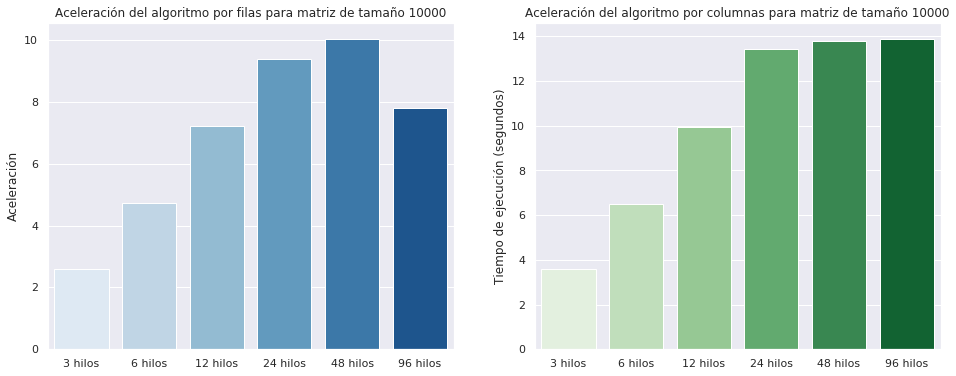
\includegraphics[width=\textwidth]{stars_accel_bar}
\label{fig:staraccelbar}
\end{figure}

En el caso de la eficiencia, vemos una historia muy parecida para ambos algoritmos.
Aunque el tiempo que toman menos tiempo real, la eficiencia del uso de recursos
en realidad baja dramaticamente aumentando el número de hilos. La figura
\ref{fig:stareff} muestra este comportamiento.

\begin{figure}[H]
  \caption{Mapa de calor de eficiencia}
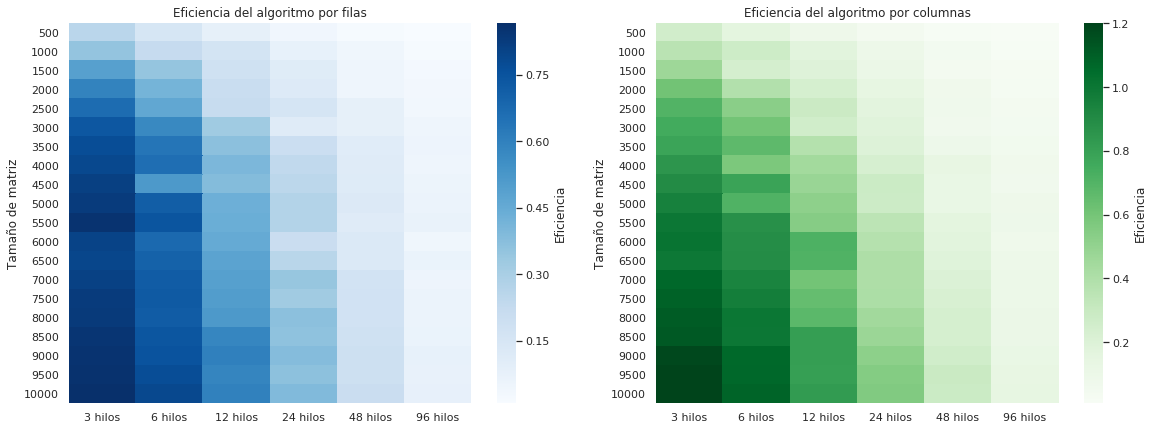
\includegraphics[width=\textwidth]{stars_efficiency}
\label{fig:stareff}
\end{figure}

En nuestra figura \ref{fig:stareffbar}, mostrando la eficiencia para nuestra mátriz
de $10000 \times 10000$, vemos como nuestra eficiencia baja constantemente,
culminando en la eficiencia con 96 hilos, que se vé dramaticamente reducida por el
tiempo gastado en cambios de contexto.

\begin{figure}[H]
  \caption{Eficiencia para mátriz de $10000 \times 10000$}
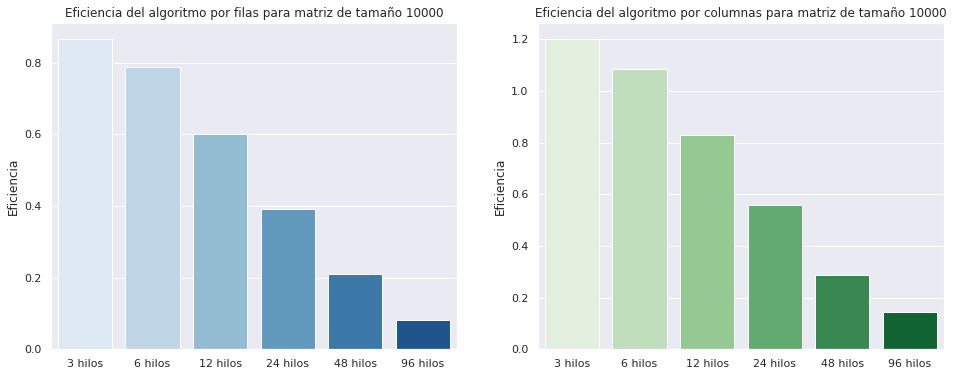
\includegraphics[width=\textwidth]{stars_efficiency_bar}
\label{fig:stareffbar}
\end{figure}

Para acabar, obervamos el overhead que sufren los algoritmos. Los resultados
son congruentes con la historia hasta ahora. El overhead aumenta con el número de
hilos, y ve un incremento dramatico en las corridas con 96 hilos. Estos resultados
estan graficados en la figura \ref{fig:staroverhead}

\begin{figure}[H]
  \caption{Overhead de los algoritmos}
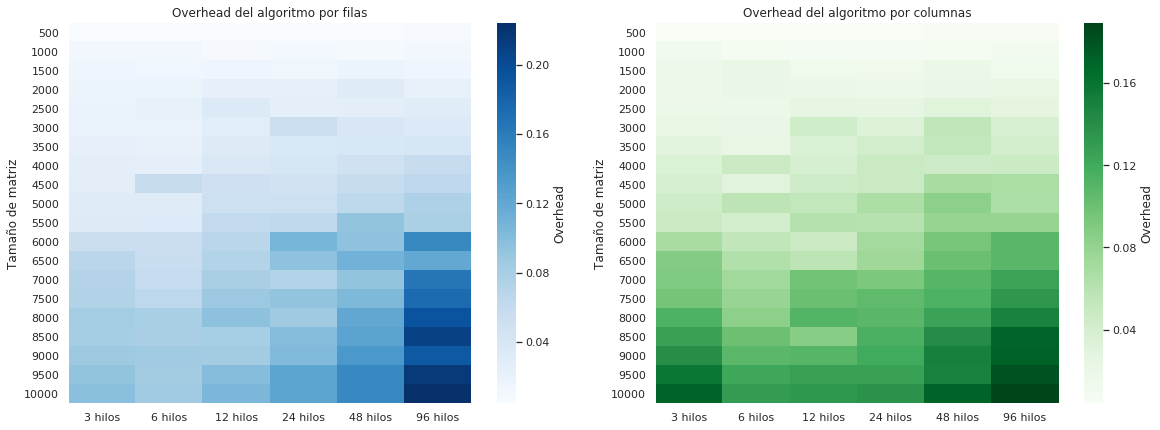
\includegraphics[width=\textwidth]{stars_overhead}
\label{fig:staroverhead}
\end{figure}

\section{Conclusión}

Ambos algoritmos de detección de estrellas nos muestran propiedades típicas de los
algoritmos distribuidos. Vemos que el algoritmo paralelo en general es mucho más
rapido que el secuencial. Pero tambien vemos que la eficiencia de uso de recursos
baja rapidamente entre mas paralelizemos el algoritmo.

Vemos tambien que hay cierto punto cuando agregar mas hilos se vuelve
contraproducente cuando la cantidad de hilos supere el numero de núcleos de
procesador con los que contamos. Este punto obviamente depende del procesador, pero
es importante estar consciente de su existencia.

\chapter{Problema 2}

\section{Descripción del problema}

\textbf{Enunciado} Analizar el desempeño del programa que calcula las raices
cuadradas entre $1$ y $n$.

\section{Descripción del algoritmo}

Los tres algoritmos son los vistos en clase:

\begin{itemize}
  \item El algoritmo secuencial original.
  \item El algoritmo paralelo usando un arreglo compartido.
  \item El algoritmo paralelo donde cada hilo regresa parte de la solución y el
    hilo principal las reune.
\end{itemize}

%
\section{Introducci\'on}
El objetivo de este trabajo es construir un algoritmo que dadas las coordenadas de dos piezas de ajedrez, de las 
cuales una es un alfil, determine si el alfil puede atacar a la otra pieza.
%
\section{Procedimiento}
Un alfil ataca a la pieza contraria si esta se encuentra en alguna de las diagonales 
Dado que cada pieza ocupa una posici\'on en el tablero es suficiente con calcular la pendiente de la recta que pasa 
por las coordenadas en las cuales se encuentran ambas piezas. 
\newline
\newline
Si el valor de dicha pendiente es $1$ o $-1$, entonces el alfil ataca a la pieza contraria.    
%
\subsection{Restricciones}
Se asume que las coordenadas de ambas piezas son v\'alidas y que cada ambas piezas no ocupan la misma posici\'on.
%
\section{Estructuras de Datos Utilizadas}
Para este problema no se ocupan estructuras de datos.
%
\section{Algoritmo}
El algoritmo para ...
\newline
\newline
{\bf Algorithm} Bootstrap
\newline
\newline
\begin{tabular}{l l}
{\bf Input}:  & $X, Y$ set of $n$ observations \\ 
              & $nbi$ Number of bootstrap iterations \\ 
              & $p$ percent of the confidence interval \\
{\bf Output}: & $x_l, x_r$ Confidence interval  \\
\end{tabular}
~~
\newline
\begin{tabular}{>{\em}r l}
\\
1 & $\rho \leftarrow \mbox{\bf CorrelationCoef}(X,Y)$ \\
2 & {\bf for}~$i~\leftarrow 1~ \mbox{\bf to}~ nbi$~ {\bf do} \\
3 & \minitab $X',Y' \leftarrow \mbox{\bf SampleFrom}(X,Y,n)$ \\
4 & \minitab $cint_i \leftarrow \mbox{\bf CorrelationCoef}(X',Y')$ \\
5 & {\bf Sort}$(cint)$ \\
6 & $x_l,x_r \leftarrow \mbox{\bf ConfidenceInterval}(cint,p)$ \\
7 & $\mbox{\bf return}~x_l,x_r$
\end{tabular}
~~~
\newline
\newline
El algoritmo primero verifica si ambas piezas se encuentran en la misma fila (l\'inea 1) o en la misma columna
(l\'inea 3); en ambos casos el resultado es {\em Fail}. 
\newline
Si ambas piezas no se encuentran en la misma fila o columna se calcula la pendiente de la recta que pasa por las coordenadas
en las cuales se encuentran ambas piezas (l\'inea 5) y luego se verifica si el valor de la pendiente es $\pm 1$ 
(l\'inea 6).
%
\subsection{An\'alisis de Complejidad}
El algoritmo propuesto tiene costo constante.
%
\section{Implementaci\'on}
El algoritmo est\'a implementado en lenguaje C como se muestra en la figura a continuaci\'on:
%\begin{figure}[h]
%\includegraphics[scale=0.5]{alfil.pdf}
%\end{figure}
\newpage
%
\subsection{Plataforma Computacional}
El programa fue ejecutado eun un computador con las siguientes caracter\'isticas:
\begin{itemize}
\item {\bf Procesador:} Intel(R) Pentium(R) 4 CPU 3.00GHz
\item {\bf Memoria RAM:} 994312 kB
\item {\bf Sistema Operativo:} Linux - Ubuntu 9.04 
\end{itemize}
%
\section{Resultados Experimentales}
En este caso es trivial ...
%
\begin{appendices}

\chapter{Datos experimentales del problema 1}

\end{appendices}


\end{document}
